\documentclass{article}
\usepackage[utf8]{inputenc}
\usepackage{DASgenerator}
\usepackage{graphicx}
\usepackage{hyperref}
\usepackage{multirow}
\usepackage[table,xcdraw]{xcolor}


%----University of Bristol Data Access Statement generator v1.2 24/10/2016----
%% DASgenerator.tex
%% Copyright 2016 University of Bristol Research Data Service
%
% This work may be distributed and/or modified under the conditions of the LaTeX Project Public License, either version 1.3 of this license or (at your option) any later version. The latest version of this license is in http://www.latex-project.org/lppl.txt and version 1.3 or later is part of all distributions of LaTeX version 2005/12/01 or later.
%
% This work has the LPPL maintenance status `maintained'.
% 
% The Current Maintainer of this work is University of Bristol Research Data Service (data-bris@bristol.ac.uk)
%
% This work consists of the files DASgenerator.sty and DASgenerator.tex

\title{Fundamentos de la Ciencia de Datos \\ PEC2: Los peligros de no gobernar los datos: calidad, seguridad y ética}
\author{Paula Muñoz Lago \\ paulamlago@uoc.edu \\ Master en Ciencia de Datos \\ Universitat Oberta de Catalunya}
\date{Diciembre 2019}
\makeindex

\begin{document}

\maketitle

\section{Gobierno de datos}

%1. Determina qué es la gobernanza de datos y su relación con la gestión de la calidad de los datos desde la perspectiva de los datos como un activo de la empresa
\subsection{Gobernanza y gestión de la calidad de datos}

Entendemos como Gobernanza de Datos el ejercicio de autoridad sobre los procesos que controlan la creación, el acceso, uso compartido, la utilización, destrucción y toma de decisiones, por ejemplo cuando surgen conflictos sobre la gestión de los activos de datos. El gobierno de datos pretende complementar a la gestión del dato, asegurando la Accesibilidad, Seguridad, Consistencia, Calidad y Auditabilidad de los datos.

%https://www.dataversity.net/data-governance-vs-data-quality-managing-data-driven-solutions/#

%2. Qué fases caracterizan la gobernanza de datos
\subsection{Fases}
Podemos resaltar hasta 7 fases en el diseño de un programa de gobernanza de datos. Si bien es cierto que cabe la posibilidad de que se tomen decisiones sobre cada fase, y la secuencia de las mismas puede no ser lineal, en función de las necesidades del proyecto.
\begin{enumerate}
	\item \textbf{Desarrollo de una descripción de valor}: Para comenzar, definiremos el valor que el programa que se va a empezar a diseñar nos va a generar, además de los margenes para la continua medición de los resultados. Basándonos en los objetivos de nuestra organización, intentaremos mejorar la misma desde un aspecto financiero a través de las ventajas que nos puede ofrecer la implementación del programa de gobierno de datos. Para identificar dicho valor, primero debemos informarnos de si ya existe algún programa funcionando y a cómo el gobierno del dato funcionará a través de estos programas.
	
	Además, debemos definir en base a qué aspectos podremos determinar que nuestro programa resulta exitoso. Por ejemplo, podremos identificar métricas financieras para conocer el resultado que obtendríamos si no dispusiéramos de \textit{Data governance}.
	
	\item \textbf{Preparación y hoja de ruta}: Se planificarán los eventos en torno al momento en la organización en el cual los datos pasan a estar gobernados. La hoja de ruta contemplará los objetivos a corto y largo plazo para alcanzar los objetivos. Como indicamos anteriormente, es preciso incluir puntos de control en los que modificar, si es necesario, el plan.
	En esta fase se integrará el gobierno de datos con otras áreas dentro de la organización, además de diseñar las métricas y generar informes para comprobar el estado del plan, definir los requisitos tanto de mantenimiento como del cambio de planificación y finalmente especificación de los detalles relativos a la puesta en marcha del programa.
	
	\item \textbf{Planificación y financiación}:
	Debemos desglosar la inversión que habrá que realizar para conseguir dicho programa, tanto en tiempo como en recursos humanos y financieros. 

	\item \textbf{Diseño}:Deberemos determinar los principios, normas y el diseño de los diferentes procesos que formarán el programa. Las actividades consistirán en identificar, documentar y aprobar qué procedimientos clave necesita la organización para empezar a considerar el dato como un activo. Además, determinaremos los procesos genéricos que sustentan los objetivos del programa. También plantearemos las responsabilidades del equipo, puesto que los procesos diseñados carecerán de utilidad hasta que no se asigne a quién le corresponde la responsabilidad. Finalmente, expondremos el modelo de \textit{Data Governance} al equipo ejecutivo para informar sobre responsabilidades y procesos.
	
	\item \textbf{Implementación}: En esta fase se pondrán en marcha los requisitos definidos durante el diseño. Tendrá, a su vez, dos sub-fases.
	\begin{enumerate}
		\item \textbf{Lanzamiento:} Momento a partir del cual la organización comienza a gobernar el dato, mientras que comienzan los procesos de información y formación en el nuevo programa a los empleados.
		\item \textbf{Cambios de plan:} Dado el soporte técnico del dato, se recogerá \textit{feedback} y tendremos que llevar a cabo dichas mejoras. Pudiendo derivar, por ejemplo, en una actualización en la guía del uso y su desencadenante nuevo plan de formación.
	\end{enumerate}
	
	\item \textbf{Gobierno}: En esta fase, deberemos incluir un marco organizativo a nuestro programa, es decir, identificar a administradores o usuarios del dato y los rangos de responsabilidad de los mismos frente al gobierno de los datos. Definiremos los niveles del marco organizativo e identificaremos los roles y responsabilidades de cada nivel.
	
	\item \textbf{Motorización, medición, creación de informes}: Necesitaremos examinar y revisar el programa periódicamente para comprobar su eficacia.


\end{enumerate}

\subsection{Componentes}
\label{componentes}
Existen diferentes componentes que conforman el gobierno de datos.
% /home/paula/Documentos/Personal/Máster/Fundamentos de la ciencia de datos/Bloque 2/PEC 2/componentes
% "/home/paula/Documentos/Fundamentos-de-la-ciencia-de-datos/Bloque 2/PEC 2/componentes

\begin{figure}[h]
	\centering
	\includegraphics[width=\linewidth]{"componentes"}
	\caption{Componentes del Gobierno de Datos}
	\label{fig:componentes}
\end{figure}

\begin{itemize}
\item \textbf{Arquitectura de Datos:} Se trata de las arquitecturas y procesos que forman parte de la arquitectura empresarial que procesan los datos.
\item \textbf{Diseño y modelo de Datos:} Consiste en gestionar, analizar, diseñar, construir, testear y mantener los modelos de datos.
\item \textbf{Almacenamiento de Datos:} Gestionar las infraestructuras físicas de almacenamiento de datos.
\item \textbf{Seguridad de Datos:} Asegurar el acceso a los datos apropiados, manteniendo así la privacidad y confidencialidad.
\item \textbf{Datos maestros y de referencia:} Identificar, mantener, gestionar, y propagar los datos maestros.
\item \textbf{Inteligencia de negocio y almacenes de datos:} Gestionar la gestión de procesos y del eficacia de acceso a la información para tomar una decisión.
\item \textbf{Integración e interoperabilidad de datos:} Gestionar todos los procesos que impliquen datos, desde su adquisición, pasando por la extracción, transformación, movimiento, propagación, replicación y federación hasta visualización de los mismos.
\item \textbf{Contenido y documentos:} Para permitir la interoperabilidad con datos estructurados, almacenaremos e indexaremos el acceso de datos en documentos.
\item \textbf{Metadatos:} Recopilación, categorización, mantenimiento,integración, control, gestión y distribución de los metadatos.
\item \textbf{Calidad del dato:} Consiste en definir, monitorizar, mantener y mejorar la calidad del dato.

Toda plataforma tecnológica de gobierno de dato debe cubrir las funciones descritas en mayor o menor medida. En el caso en el que una organización disponga de departamento de seguridad tecnológica, sobre el cual recae la responsabilidad de la función de seguridad del dato, deberemos coordinar todas las funciones.


\end{itemize}
\subsection{Impacto del gobierno de datos en la adquisición de ONO por Vodafone}
Dado un programa de gobierno de datos ya definido en Vodafone, deberemos integrar los datos provenientes de ONO en nuestro sistema, para ejercer autoridad sobre ellos también. 

Dado que los clientes de ONO tendrán el mismo nivel de importancia que los que ya eran clientes de Vodafone, debemos entender cómo funcionaran estos datos con los programas que ya están funcionando.

También deberemos replantear la \textbf{hoja de ruta}, para planificar nuevos eventos en torno al momento en el que los datos provenientes de ONO pasarán a estar gobernados. También deberemos hacer una planificación del esfuerzo que supondrá la ampliación de la gobernabilidad tanto en recursos financieros como humanos y temporales.

Para poder considerar estos nuevos datos como activos de Vodafone, tendremos que \textbf{adaptar el diseño} previamente establecido, puesto que quizás necesitemos nuevas funcionalidades o miembros del equipo con nuevas responsabilidades. En último lugar, si se han dado cambios, debemos establecer un \textbf{nuevo plan de formación} para informar debidamente a los miembros del equipo.

Como  mencionamos anteriormente, parte de la integración total de los nuevos datos consiste en \textbf{identificar a los nuevos usuarios} y la necesidad de crear \textbf{nuevas responsabilidades} sobre los nuevos datos.


\subsection{Propuesta de organización que cubre las funciones DAMA}
Para comenzar, \href{https://dama.org/}{DAMA}, o \textit{Data Management Association} es una asociación internacional de profesionales focalizados en los conceptos y prácticas relativos a la gestión del dato y de la información, y cuyo modelo es el  \href{https://dama.org/content/body-knowledge}{DMBook}. 

Aplicaremos las características DAMA a una librería online que quiere gobernar sus datos, previamente disponían de una gestión interna para indexar y organizar los libros de los que disponían. Actualmente, van a dar el paso a abrir una tienda online.

Dado que dicha librería quiere cubrir de todos los componentes DAMA mencionados anteriormente (Punto \ref{componentes}), la definiremos como una empresa que quiere ejercer una autoridad sobre los datos, gobernándolos, y tratar sus datos como activos de la organización. La \textbf{arquitectura de datos} estará conectada con los objetivos de la librería, ayudando a la misma a conseguir sus objetivos. Además, la arquitectura de los datos procedentes de la nueva tienda online ha de disponer de un plan de integración con la arquitectura existente, ya que es crucial que funcione en conjunto con lo anterior para lograr la gobernabilidad del dato.
La clave para que la arquitectura de datos de esta organización ficticia funcione, será que disponga de una estrategia de implementación y que sea manejable. \footnote{\url{http://informatica.blogs.uoc.edu/2016/12/19/data-governance/}}.

En cuanto a la función de \textbf{Diseño y modelado de datos}, nuestra empresa tendrá un equipo encargado de definir la estructura lógica de una base de datos, y habrán definido cómo los datos se conectan entre sí, procesan y almacenan. Por ejemplo, deberán diseñar los datos y podrán determinar que el modelo más adecuado para representar los mismos sea el modelo entidad relación.
\begin{table}[h]
	\centering
	\begin{tabular}{lcc}
		\rowcolor[HTML]{3531FF} 
		\cellcolor[HTML]{FFFFFF}                            & \multicolumn{1}{l}{\cellcolor[HTML]{3531FF}Libro} & \multicolumn{1}{l}{\cellcolor[HTML]{3531FF}Usuario} \\
		\cellcolor[HTML]{3166FF}                            & \textbf{ISBN}                                     & e-mail                                              \\
		\cellcolor[HTML]{3166FF}                            & Título                                            & usuario                                             \\
		\multirow{-3}{*}{\cellcolor[HTML]{3166FF}Atributos} & Autor                                             & contraseña                                         
	\end{tabular}
	\caption{Ejemplo de diseño de datos}
	\label{tdiseno}
\end{table}

En la tabla \ref{tdiseno} se expone un ejemplo de diseño de algunos datos relevantes en la librería, como un libro, que tendrá como atributos el ISBN que será su clave única con el que se podrá referenciar y el usuario, cuya clave única será el e-mail.

\begin{figure}[h]
	\centering
	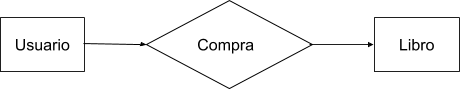
\includegraphics[width=0.7\linewidth]{er}
	\caption{Ejemplo de relación "compra"}
	\label{fig:er}
\end{figure}

La figura \ref{fig:er} muestra un ejemplo de una relación que tiene que estar reflejada en el modelo, ya que será lo que impulse el objetivo final de la empresa. La relación compra será llevada a cabo por un usuario, y deberá elegir uno o más libros.

En cuanto al \textbf{almacenamiento de los datos}, la librería deberá disponer de algún servidor en el que alojar su base de datos, tanto de forma local como en la nube. Además, deberán asegurarse de la \textbf{seguridad del sistema}, ya que han de conservar la privacidad y confidencialidad de los nuevos datos que se incorporan a su sistema como los de sus usuarios. Así como asegurar la falta de vulnerabilidades en la página web que crearán.
Existen diferentes empresas que ofrecen un servicio de hosting de base de datos, como \href{https://aws.amazon.com/es/products/databases/}{Amazon}.

Como parte del proceso de gobernar los datos de los que han pasado a disponer, deberán identificar cuales son sus \textbf{datos maestros y de referencia}, además de mantenerlos, gestionarlos y determinar una forma de acceder a ellos. Los datos mostrados en la tabla \ref{tdiseno} podríamos considerarlos datos maestros, ya que son un conjunto de información relacionada con el producto o con el usuario de nuestra empresa. Además, son datos transaccionales, que no cambian tras realizar una operación. Por ejemplo, una entrada del tipo usuario no se verá modificada tras realizar una compra. Por otra parte, los datos de referencia podrían considerarlos los datos que definen el movimiento, como el identificador de compra. 
Los \textbf{Metadatos}, sin embargo, son datos que se recopilarán de los movimientos producidos, como la compra de un libro. Esto conlleva la categorización, mantenimiento, control y distribución de los mismos.

Para implementar una \textbf{Inteligencia de negocio}, deberán gestionar los procesos que analizan los datos de la librería. Por ejeplo, pueden analizar los datos del historial de compras por temporadas y predecir qué libro se venderá más en base a las características de cada uno, con el fin de publicar ofertas en el precio.

Con el fin de simplificar los movimientos, la librería dispondrá de una \textbf{Integración e interoperabilidad de datos}, es decir, será capaz de integrar datos heterogéneos de diferentes fuentes, transformando o replicando los datos si fuese necesario. Por ello, una vez disponga de un conjunto de usuarios registrados en el sistema de compras en su base de datos, podrá integrar los datos que recibe el sistema de la pagina web con la base de datos para comprobar si el usuario ya dispone de cuenta en el sistema o no. También, podrán visualizar los datos que necesiten entender con más facilidad, como el número de ventas por mes, trimestre, o año. En la figura \ref{fig:facturacion-por-materias-1024x785} observamos la visualización de los tipos de libros que se vendieron en 2018 \footnote{\url{http://wmagazin.com/la-venta-de-libros-en-espana-se-estanca-en-el-pais-y-crece-en-el-exterior/}}.

\begin{figure}
	\centering
	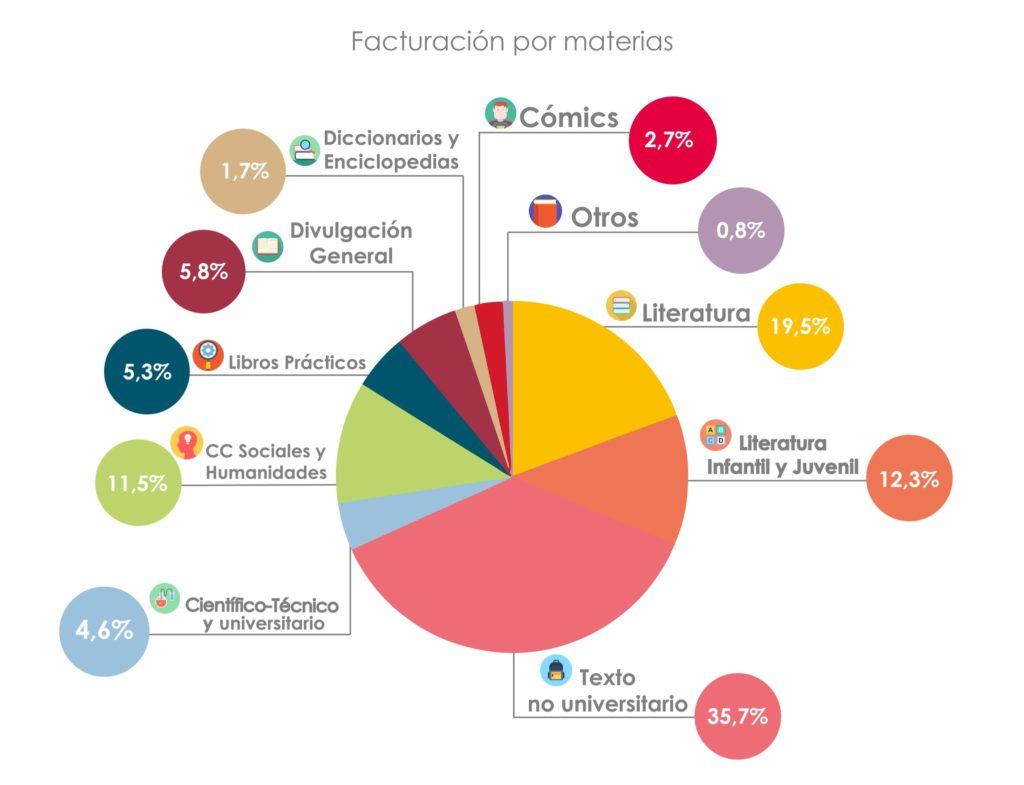
\includegraphics[width=0.8\linewidth]{facturacion-por-materias}
	\caption{Venta de libros en España en 2018}
	\label{fig:facturacion-por-materias-1024x785}
\end{figure}



Los trabajadores de esta librería deberán almacenar, proteger, indexar y habilitar el acceso a los datos. Además, generarán informes y documentos detallando el uso de las nuevas herramientas integradas en la empresa.

Finalmente, definirán la \textbf{calidad de los datos}, por ejemplo, que la clave única que referencia a los libros, el ISBN,debe tener siempre el mismo número de dígitos, y de no ser así, se rellenará con ceros a la izquierda, mientras que la clave única del usuario debe contener el carácter '@', de esta forma se conseguirá una mejor calidad e integración de los datos con la arquitectura existente.
 
%https://dama-ny.com/images/meeting/101608/datagovernmodelingbestpractices.pdf

%http://informatica.blogs.uoc.edu/2016/12/19/data-governance/
%https://www.gub.uy/agencia-gobierno-electronico-sociedad-informacion-conocimiento/comunicacion/noticias/uruguay-politica-datos-para-transformacion-digital?idPadre=1937
%https://centroderecursos.agesic.gub.uy/web/arquitectura-de-gobierno/arquitectura-integrada-de-gobierno/-/wiki/Arquitectura+de+Gobierno/Modelo+de+Referencia+de+Datos

\section{Relación del gobierno de datos con la RGPD}
\subsection{¿Cómo deben gobernarse estos datos? ¿De qué manera hubiese afectado al gobierno de datos el RGPD?}
\label{2.1}
%¿Cómo deben gobernarse estos datos? METADATOS
Dado que además de los datos proporcionados mediante el contrato, Vodafone está recogiendo también datos de red, información del origen, destino y duración de las llamadas y datos de geolocalización, deberán notificar a sus nuevos clientes provenientes de ONO de la actualización en el uso de sus datos. De no ser así, estarían incumpliendo la RGPD. Sin embargo, Vodafone no sería la única empresa Española que caería en tal incumplimiento. Según la aportación de un compañero en el foro de la asignatura, en la que incluye la "lista de culpables del GDPR", otros compañeros han debatido sobre la presencia en esa lista de \textit{La Liga} Española de Fútbol. Ésta empresa recogía datos de las personas que tenían descargada su aplicación sin notificarles nada con fines propios, por lo que ha recibido una multa. De esta forma, podemos concluir que, basándonos en esta aportación del debate, Vodafone sería multada de recoger tales datos sin conocimiento de la totalidad de sus usuarios.
Dentro del contexto del gobierno de datos, interpretar el contexto de los datos dado por los metadatos de los mismos es crucial para administrarlos de la mejor manera posible. Para gobernar estos metadatos generados, por ejemplo, del establecimiento de una llamada, la empresa deberá, además de notificar al usuario su recopilación como se explica anteriormente, mantenerlos, gestionarlos e integrarlos en el sistema \footnote{\url{https://blog.powerdata.es/el-valor-de-la-gestion-de-datos/la-importancia-de-los-metadatos-en-el-gobierno-de-datos}}. Su distribución en la empresa también se verá afectada por la RGPD. 

%¿De qué manera hubiese afectado al gobierno de datos el RGPD
El RGPD regirá desde la unidad mínima del gobierno de datos, el dato convertido en activo de la empresa, hasta procesos y personas, pasando por las comunicaciones externas a la organización e internas .
Tras la implantación del RGPD, los componentes del gobierno de datos se ven modificados, algunos de los aspectos clásicos sobre los que se asienta el gobierno de los datos corporativos tendrán que revisarse ahora, para adaptarlos al nuevo Reglamento europeo. Por ejemplo, se deben incluir medidas organizativas como incorporar el rol de delegado de protección de datos, generación de registros de actividades de tratamiento de datos, como inventarios internos y establecer políticas de protección de datos más exhaustivas. Además, tras la implantación del reglamento, sumamos la toma de conciencia y compromiso al trabajar y ser responsables de datos personales.
\footnote{\url{https://blog.es.logicalis.com/analytics/gobierno-de-los-datos-y-gdpr-rgpd-dos-caminos-convergentes}} \footnote{\url{https://www.abogacia.es/2018/05/07/de-la-proteccion-del-dato-al-gobierno-del-dato-pasando-por-el-rgpd/}}.

Cualquier empresa debe tener en cuenta los aspectos que rigen el RGPD, que como comenté en mi aportación al debate, se resumen en:
\begin{itemize}
\item  Acceso a la información del tratamiento de nuestros datos personales para conocer con qué fin se están utilizando.
\item Oposición, ofreciendo al usuario la posibilidad de negarse a que la empresa utilice sus datos.
\item Rectificación, dado que si un usuario encontrase algún dato erroneo, deberá disponer de la posibilidad de cambiarlo.
\item Supresión, además de poder cambiar un dato, la empresa ha de ofrecer la posibilidad de borrarlo.
\item Portabilidad de los datos, es decir, la empresa debe estar dispuesta a entregar al usuario los datos.
\item Limitación del tratamiento, otorgar la posibilidad al usuario de determinar para qué quiere que se usen sus datos y para qué no.
\end{itemize}

\subsection{Relación con el triángulo de la seguridad}
El Triángulo de la seguridad, también denominada Tríada CID o \textit{CIA Triad} en Inglés, se refiere a tres principios que deben trabajar en conjunto para garantizar la seguridad de un sistema informático: Confidencialidad, Integridad y Disponibilidad. Se trata de un modelo diseñado para guiar las políticas de seguridad de la información dentro de una organización. A continuación, se desarrollará cada concepto.
\begin{itemize}
\item \textbf{Confidencialidad}: Medidas emprendidas para evitar que la información privada llegue a las personas equivocadas, mientras que las personas que necesitan dicha información pueden acceder a ella de forma segura y restringida. Algunas técnicas para mantener la confidencialidad puedes ser el cifrado de datos, además de la identificación del usuario, mediante una contraseña o verificación biométrica, tokens etc.
\item \textbf{Integridad}: Consiste en mantener la precisión, confiabilidad y consistencia de los datos durante su ciclo de vida. Es decir, que no se vean alterados ni en almacenamiento, ni en proceso, ni en tránsito. Para ello podemos usar programas de control de versiones para evitar cambios o eliminaciones no deseadas, como \href{https://github.com/}{GitHub}.
\item \textbf{Disponibilidad}: Todos los usuarios autorizados a disponer de dicha información deben poder acceder a ella en cualquier momento. Para ello hay que tener planificadas recuperaciones ante pérdidas de datos, interrupciones en las conexiones. Para ello se puede guardar un back-up en un lugar geográfico diferente a dónde se alojan los datos normalmente.
\end{itemize}

Dada esta información, a la hora de adquirir una nueva compañía o crear una nueva, se han de tener en cuenta estos aspectos, además de los presentes en el nuevo RGPD, los cuales están incluidos en la sección de Confidencialidad de la Tríada CID. La utilización del triángulo de seguridad en una organización para la clasificación de la confidencialidad, integridad y disponibilidad de los recursos cibernéticos ayuda a determinar el riesgo para la institución y a dar un cierto valor a la protección de los datos. \footnote{\url{https://www.ontek.net/que-es-triada-cid/}}
\footnote{\url{https://blog.smartekh.com/que-es-la-triada-de-seguridad-o-cia-triad-y-por-que-deberia-interesarte}}
\footnote{\url{https://donnierock.com/2018/03/12/que-es-la-triada-cid-o-el-triangulo-de-la-seguridad/}}
\footnote{\url{https://www.al-enterprise.com/-/media/assets/internet/documents/campus-security-whitepaper-es.pdf}}
\subsection{Identidad y privacidad}

La anonimización de los datos persigue ocultar la identidad y la información sensible de los usuarios que aparecen en los conjuntos de datos, en este caso, los usuarios de ONO, ahora de Vodafone. Las técnicas de anonimización existentes buscan hacer a un individuo único en un conjunto de datos, ocultando sus detalles. Encriptando la información de tal forma, si hubiese un ataque, el atacante solo podría deducir la información en base a una probabilidad.

Existen diferentes modelos de protección:
\begin{itemize}
	\item \textbf{Aleatorización}: Consiste en alterar los datos introduciendo ruido en los originales, sin elevar mucho el nivel de perturbación ya que podemos terminar generando datos aleatorios. El punto débil de este modelo es que no preserva los valores de los outliers.
	\item \textbf{K-anonimidad}: Asegura que un usuario no podrá ser distinguido de otros k-1 usuarios presentes en el mismo conjunto. Se lleva a cabo generalizando cada k valores los atributos de los datos. La ventaja de esta técnica es que el atacante puede descifrar los datos con una probabilidad menor a 1/k, por otra parte, el valor k es dado por el nivel de privacidad con el que se quierda dotar al conjunto. Al aumentar su valor se reduce su utilidad dada la falta de precisión.
	\item \textbf{Privacidad diferencial}: Introducida para proteger los resultados de las consultas a una base de datos. La anonimización se sitúa entre el usuario que ejecuta las consultas y el controlador de base de datos. Para mantener la privacidad de los individuos, se debe considerar que la aportación de datos de un individuo al conjunto es limitada. Es una condición en la publicación de datos, no en el propio conjunto.
\end{itemize}

En el caso de la privacidad de datos como el destino y origen de las llamadas o su duración, tratado en el punto \ref{2.1}, podemos convertir cada metadato a un número u otro identificador que sea conveniente, para a continuación proceder con un método de enmascaramiento para datos numéricos. En el caso de que existiese la posibilidad de convertir los datos a variables categóricas, también podremos enmascarar los datos haciendo uso de las mismas.

Podemos relacionar los conceptos de identidad y privacidad con la tríada CIA, ya que anonimizar los datos mejora la confidencialidad de los mismos, ya que añade más seguridad. Identificarlos correctamente ayuda a mantener la Integridad de éstos, ya que de otra forma puede darse una pérdida de consistencia, mientras que estén a disposición de todos los usuarios que tengan acceso a ellos, y puedan \textit{desenmascararlos} y observar sus atributos.

\section{Mercado de Datos}
\subsection{Qué son}
Un Mercado de datos es una plataforma de compra y venta de datos. Ponen en contacto a empresas que tienen datos para venderlos a empresas más pequeñas, como startups, que los necesitan. Además, no hacen únicamente de intermediarios, también ofrecen maneras de localizar los conjuntos de datos y dan indicaciones sobre la calidad de los mismos, proporcionando APIs que permiten acceder a ellos, por ejemplo, a \textit{Data brokers}. Algunos de los mercados más famosos son \href{https://www.datapace.io/}{Dataplace},  \href{https://www.qlik.com/us/products/qlik-data-market}{Qlik DataMarket} o la empresa española \href{https://www.taptapnetworks.com/}{TapTap}, cuyo producto principal es Sonata. Este programa se basa en la geolocalización para ofrecer información a nivel mundial a partir de datos tanto públicos como privados. Indica cuál es el gasto medio de las tarjetas de crédito en cada área, qué se está comentando en redes sociales, el nivel de tráfico a esa hora, rangos de edad de las personas que pasan por allí, sus estados de ánimo o  el índice de natalidad en la manzana. Debemos destacar el ejemplo de las teleoperadoras que nos ofrecen servicios de internet en nuestros dispositivos móviles, éstas, antes de vender nuestros datos, los anonimizan e integran en una base de datos junto con la ubicación y el tiempo real. Estos datos se denominan \textit{Datos agregados}, ya que no se puede identificar a un usuario basándose en ellos.

En conclusión, los mercados de datos son un negocio emergente en internet y su ploriferación hará que cada vez sea más fácil conseguir datos de calidad y abrirá oportunidades de generar ingresos a partir de nuestros datos.\footnote{\url{https://jmalarcon.es/posts/Compra-y-venta-de-datos-el-siguiente-gran-negocio-en-Internet}} \footnote{\url{https://www.eldiario.es/tecnologia/trabaja-empresa-compra-venta-personales-sentido_0_955054905.html}}.


%http://dataanalysis.blogs.uoc.edu/2018/02/15/el-mercado-de-datos-siempre-en-evolucion/
%https://www.3ciencias.com/wp-content/uploads/2014/02/MERCADOS-DE-DATOS-PARA-EL-AN%C3%81LISIS-ESTAD%C3%8DSTICO-DE-LA-INFORMACI%C3%93N2.pdf
\subsection{Cómo se gobiernan los datos de uno o más mercados}
Para gobernar los datos de un mercado, debe cumplir todos los componentes DAMA. Dado que los datos presentes en dichos mercados son multidimensionales, es decir, estarán compuestos de más de un atributo, su \textbf{arquitectura} será multidimensional. Existen diferentes \textbf{diseños y modelos de datos} disponibles para éstos datos y sus \textbf{Metadatos}, que aportarán el contexto de éstos, como el esquema estrella, que relaciona diferentes tablas teniendo en el centro de ellas una tabla central con sus respectivos identificadores. El \textbf{Almacenamiento de estos datos} se llevará a cabo en bases de datos multidimensionales, en las cuales podremos reacomodar la orientación dimensional de una o varias tablas ejecutando una rotación haciendo uso de técnicas como \textit{Roll-up} y \textit{Drill-down}. La \textbf{Seguridad de datos} es crucial al tratar con tal cantidad de datos de índole personal en la mayoría de casos, por lo que uno de los pasos principales a tener en cuenta es diferenciar los \textbf{datos maestros y los de referencia} en nuestro conjunto, y así aplicar \textbf{Inteligencia de negocio}, gracias a herramientas como \textbf{OLAP}, que permiten el análisis de datos de forma interactiva. Ésta herramienta permite la \textbf{Integración e interoperabilidad de datos}, ya sean provenientes de una o varias fuentes, en este caso, mercados de datos, y puede \textbf{almacenar} millones de datos con relaciones complejas, manteniendo la arquitectura multidimensional planteada anteriormente, así como la \textbf{Calidad} de los mismos. Dado que necesitamos dicha arquitectura, el tipo de herramienta OLAP se llamará MOLAP, que incluirá una arquitectura compuesta por una base de datos de más de una dimensión y un motor analítico \footnote{\url{https://dialnet.unirioja.es/servlet/articulo?codigo=4835866}}.

\subsection{Procesos de anonimización de los datos de los mercados}

Previamente a la publicación de datos en un mercado, se ha procedido a su anonimización, rompiendo el vínculo entre la persona y el dato en cuestión, para así cumplir la RGPD \footnote{\url{https://www.publico.es/sociedad/tecnologia-demuestran-datos-personales-anonimizados-no-garantizan-privacidad.html}} . Existe el riesgo de poder revertir dicha anonimización, reidentificando así a la persona \footnote{\url{https://blog.psnsercon.com/la-anonimizacion-de-datos-es-facilmente-reversible-segun-un-estudio/}}.

En este caso, las técnicas de anonimización pueden ser de datos tabulares, ya que la empresa que vende los datos entrega un conjunto en una o varias tablas, las cuales deben anonimizarse conjuntamente. Existen métodos de enmascaramiento de varios tipos, \textbf{perturbativos}, que modifican el conjunto original de algún modo, por ejemplo, introduciendo ruido en algún atributo, alterando su valor. Otro tipo de enmascaramiento son los métodos \textbf{no perturbativos}, que se logra sustituyendo el valor original por otro menos específico, más general. Por último existen los \textbf{generadores de datos sintéticos}, que en lugar de distorsionar los datos originales, crean nuevos datos para sustituirlos, a partir del conjunto original. Por ejemplo, podemos sustituir la duración de las llamadas de los clientes de una compañía por valores generados a partir de la media y varianza de los originales.

Generalmente, todos estos métodos cumplen la k-anonimidad, condición que debe ser satisfecha para todo conjunto de datos protegido. Mantiene que para cualquier combinación de atributos existen k o más registros que comparten los mismos valores.

\subsection{Relación anonimización, ciclo de vida y valor de los datos}
La anonimización de los datos debe ser controlada, ya que si se generaliza mucho sus atributos o se perturban en exceso, puede darse una pérdida de utilidad en los mismos. Por ejemplo, en la k-anonimidad mencionada anteriormente, cuanto más aumenta el valor k, más aumenta su privacidad y se reduce su utilidad. En general, podremos medir el valor de un dato basándonos en el coste del mismo, es decir, el precio pagado en un mercado de datos para adquirir el mismo. También podemos basarnos en el mercado, es decir, el precio que un tercero podría pagar ahora mismo, o basándonos en su utilidad. Estos tres métodos para valorar un dato están influenciados por la previa "encriptación" de los mismos para dotarlos de anonimidad.

Como parte del ciclo de vida de los datos, tenemos que introducir la privatización de los mismos, para cumplir con los requisitos y los reguladores del país en el que se opera, en este caso basándonos en el RGPD. Deberemos ayudar a proteger los datos sensibles mediante la gestión de acceso a los mismos, alinear la arquitectura de seguridad e iniciativas de negocio, asesorar y gestionar el riesgo, cumplir los requisitos reguladores e identificar al personal involucrado.


\subsection{Influencia de la ética en la venta de datos personales}
Existen diferentes teorías éticas que definen su quehacer como "pensamiento moral", y éticas aplicadas, entre las que se incluye la ética profesional, más orientadas en orientar en la toma de decisiones. No se tratan de normas, sino de principios que ayudan a los profesionales del sector a evaluar cuánto de bueno y realizable o malo y evitable hay en una acción. Por ello, a la hora de vender datos personales en un mercado de datos, hay que tener en cuenta varios principios. \textbf{Principio de beneficencia}, puede entenderse en términos de utilitaristas, donde se identifica el bien y la finalidad de la acción profesional. Éste principio entra en conflicto con el \textbf{Principio de autonomía}, que evalúa la instrumentación o no de las personas al cumplir tal objetivo. Considerar la autonomía implica el respeto por la dignidad individual, asumiendo que cada individuo somos un fin en nosotros mismos y no un mero medio para alcanzar un fin. En este caso, este principio sería el más relevante a la hora de estudiar la ética en la venta de datos personales, ya que, pese a que por ley deban estar anonimizados, la posibilidad de rehacer tal privatización genera incertidumbres éticas. Habrá que estudiar si se estaría tratando a un individuo, generador del dato, como un medio para conseguir un fin (dinero), o el individuo está totalmente desvinculado del dato. Dado que los principios anteriores han entrado en conflicto en el caso propuesto, se debe recurrir al \textbf{Principio de justicia}, que nos permitirá ordenar y jerarquizar las posibilidades de acción de acuerdo con criterios de justicia social. Por último, deberemos recurrir al \textbf{Principio de no maleficiencia}, al cual recurriremos en última instancia si los anteriores no han sido clarificantes, que indica: "ante todo, no hacer daño".

En conclusión, la proliferación de los mercados de datos y el movimiento en sus plataformas dificulta que los usuarios puedan ejercer su derecho a corregir los errores o falsedades que alberguen dichos datos. En consecuencia, al otorgar acceso a estas tecnologías, se genera un riesgo elevado para que se implante la tiranía en nuestra democracia. Dado que no hay barreras de intrusión, hay agencias gubernamentales de investigación con tendencia a violar las expectativas de privacidad.

\section{Terminología}
\subsection{Calidad VS gobierno de datos}
Asegurar la calidad de los datos es un paso previo a la instauración de un gobierno de datos, ya que la calidad de los datos asegura que éstos puedan considerarse un activo para la organización. Podemos definir la calidad de datos como un grado en el que los datos cumplen un conjunto de características. Según el enfoque DAMA, las dimensiones de calidad son: Completitud, Unicidad, Atemporalidad, Validez, Precisión o exactitud y Consistencia.
Una buena calidad de los datos puede desencadenar en una mayor efectividad en la adquisición y retención de clientes, optimización de todos los departamentos, ejecución de procesos eficientes, eliminación de errores, penetración rápida en nuevos mercados y toma de decisiones inteligentes y oportunas. Por lo tanto, ambos conceptos están conectados. Definiremos gobierno de datos como un sistema de decisiones y responsabilidades sobre procesos de información ejecutados de acuerdo a unos modelos que describen quién puede tomar qué decisiones, usando una cierta información y bajo unas circunstancias concretas. Por ello, cualquier intervención manual en un proceso de flujo de datos puede derivar en un error dada una baja calidad de los mismos. También si se utilizan sistemas no sincronizados que deben compartir información, o tras aplicar una fórmula u algoritmo incorrecto sobre los datos. Además se corrompe la calidad del dato al enviar informes desfasados, o al albergar metadatos que describen los datos de manera incorrecta.

Es por ello que la calidad de los datos es crucial en el gobierno de los mismos, mientras que cualquier fallo en los procesos que componen dicho gobierno pueden alterar la calidad de éstos y derivar en fallos o en pérdida de eficiencia. Si los datos fuesen agua, el gobierno de datos sería el grifo, encargado de repartir agua a las personas así como establecer las cantidades y las personas adecuadas, mientras que la calidad del agua, o en nuestro ejemplo, la calidad de los datos, sería la depuradora, encargada de que el agua no esté contaminada.

\subsection{Calidad VS madurez}
Para crear un programa de calidad de datos, que evalúa la calidad de los datos dentro de una organización, identificando los atributos más representativos y analizándolos en su contexto actual o futuro y proporcionar una guía para la mejora de la calidad de los mismos, habrá que basarse en la madurez de nuestra organización, en base a la situación en la que nos encontramos. El nivel de madurez de una empresa se mide por sus procesos internos y las personas que están al mando de identificar los datos de baja calidad o defectuosos. Además, el nivel de madurez se divide a su vez en cinco estados. Desde el \underline{inicial}, en el que no hay calidad del dato, se impone una solución \textit{ad hoc}, en la que se elabora una respuesta a un problema de forma puntual, y no es generalizable, hasta \underline{optimizado}, en el que hay un programa totalmente integrado en todos los procesos midiendo la calidad de los datos utilizados. Además, existen estados intermedios como \underline{repetible}, en el que se identifican las fuentes con datos de baja calidad, \underline{definido}, en el cual ya se ha implementado un entorno que monitoriza la calidad del dato, y \underline{gestionado}, en el cual ya se evalúa y mide el impacto de la calidad de los datos.

\subsection{Cómo se puede medir y mejorar la calidad de los datos}
Existen diferentes medidas que determinan la calidad de los datos, detalladas a continuación. \footnote{\url{https://www.whitepapers.em360tech.com/wp-content/files_mf/1407250286DAMAUKDQDimensionsWhitePaperR37.pdf}} \footnote{\url{https://blog.powerdata.es/el-valor-de-la-gestion-de-datos/bid/368790/las-6-dimensiones-de-la-calidad-de-los-datos}}.

Las medidas cuantitativas son:

\begin{itemize}
\item \textbf{Coherencia:} Los datos mostrados en las tablas deben estar en un formato legible, estándar, y coherente.
\item \textbf{Integridad:} Mide la ausencia de diferencia al comparar dos o más representaciones frente a su definición.
\item \textbf{Completas:} Medida de la ausencia de valores vacíos o nulos o la presencia de valores útiles.
\item \textbf{Oportunas:} Mide el tiempo que tardamos en disponer de los datos.
\item \textbf{Accesibles:} Medición que determina la comprensión, utilización y facilidad de acceso a los datos.
\item \textbf{Validez:} Medida que determina si un dato es conformado por una cierta sintáxis (formato, tipo o rango), dada su definición.
\item \textbf{Precisión:} Grado en el cual los datos describen correctamente el objeto o evento estudiado.
\end{itemize}

Mientras que también se deben tener en cuenta medidas cualitativas, como:
\begin{itemize}
\item \textbf{Satisfacción de negocio}: Aumento o disminución en la satisfacción del negocio con la mejora en los datos.
\item \textbf{Productividad:} Porcentaje de veces que el consejo de gobernanza de datos detectó y eliminó proyectos redundantes.
\item \textbf{Oportunidad de negocio y medidas de riesgo:} Miden el beneficio y aumento de competitividad dado el aumento de la calidad de los datos.
\item \textbf{Medidas de cumplimiento:} Permiten entender el comportamiento de los usuarios respecto a sus niveles de acceso a los datos.
\end{itemize}

Las medidas siempre se podrán ajustar a las necesidades de la organización y a su gobierno de datos. Para poder mejorara la calidad de los datos, previo a la instauración del programa de calidad de datos, se deben establecer las expectativas a la hora de mejorar la calidad, pero no sólo desde un ámbito técnico, sino tiene que estar vinculado a la satisfacción de las expectativas de negocio. Para ello habrá que haber identificado los impactos empresariales, sus problemas y causas y cuantificar los costes para eliminar los problemas relacionados con datos y beneficios asociados.


\subsection{Funciones y roles. Propietarios de datos VS administradores de datos}
El administrador de los datos es responsable en última instancia de la gestión de datos como un activo corporativo, hace el seguimiento de datos dentro de la organización y refuerza las reglas internas de cómo han de usarse los datos, mantiene las definiciones y formatos de datos acordados e identifica inconvenientes en la calidad de los mismos \footnote{\url{https://medium.com/data-management-en-espa\%C3\%B1ol/data-stewardship-52a2d46d30be}}. Por otra parte, el dueño de los datos conoce el riesgo de hacer un uso indebido de los datos, sobretodo los de índole personal. Otorga acceso a personas concretas a los datos y se lo restringe a otras.

\end{document}

